\documentclass[12pt,a4paper]{article}

\usepackage[a4paper, top = 2cm, bottom = 2cm, left = 1.5cm, right = 1.5cm]{geometry}
\usepackage[dvipsnames]{xcolor} % Colors

\usepackage{standalone}

\usepackage{setspace}
\usepackage{graphicx}
\usepackage{amsfonts}
\usepackage{amsmath}
\usepackage{tikz}
\usepackage{pdfpages}
\usepackage{epigraph}
\usepackage{csquotes}
\usepackage{natbib}
\usepackage{listings}
\usepackage{physics}
\usepackage{subcaption}

\definecolor{dkgreen}{rgb}{0,0.6,0}
\definecolor{gray}{rgb}{0.5,0.5,0.5}
\definecolor{mauve}{rgb}{0.58,0,0.82}

\lstset{frame=tb,
  language=Matlab,
  aboveskip=3mm,
  belowskip=3mm,
  showstringspaces=false,
  columns=flexible,
  basicstyle={\small\ttfamily},
  numbers=none,
  numberstyle=\tiny\color{gray},
  keywordstyle=\color{blue},
  commentstyle=\color{dkgreen},
  stringstyle=\color{mauve},
  breaklines=true,
  breakatwhitespace=true,
  tabsize=3
}

% Bibliography
\usepackage{xcolor}
\usepackage{hyperref}
\hypersetup{
colorlinks=true,
citecolor=MidnightBlue,
linkcolor=MidnightBlue,
pdfpagemode=FullScreen}

\usepackage{natbib}
\usepackage[noabbrev]{cleveref}
\setcitestyle{authoryear,open={(},close={)}}
\bibliographystyle{plainnat}

\usepackage{subfiles}

\setlength\parindent{0pt}
\spacing{1.2}
\setlength{\parskip}{1em}

\newcommand{\R}{\mathbb{R}}
\newcommand{\Z}{\mathbb{Z}}
\newcommand{\N}{\mathbb{N}}
\newcommand{\Q}{\mathbb{Q}}

%------------------------------------------------------------------------

\begin{document}

\begin{center}
       \vspace*{1cm}
       \huge\textbf{Project 3} \\
       \vspace{0.4cm}
       \large \textbf{Public Finance in Macroeconomics} \\
       \vspace{0.5cm}
        \large Handed in by the \textcolor{orange}{\textbf{Heterogeneous Geeks}} \\
        \vspace{0.3cm}
        a.k.a. Vivien Voigt, Thong Nguyen, 
\includegraphics[scale=0.06]{graphs/geek.png}\\Davide Difino \& Celina Proffen \\
       \vspace{1.5cm}
       \vfill



        Project in the context of Prof. Ludwig's course: \\
        \textbf{Public Finance in Macroeconomics: Heterogenous Agent Models}\\
        at the Graduate School of Economics, Finance and Management
       \vspace{0.8cm}
   \end{center}

\newpage

%------------------------------------------------------------------------

\section*{Problem 1.1}

The code simulates (N=10000) a life-cycle portfolio choice model. It plots the marginal propensity to consume and the estimated portfolio share as well as the the rate of return, consumption, assets, share invested in risky assets, portfolio return for the first simulation and means of consumption, assets, cash on hand, consumption growth, share invested in risky assets, protfolio return over an individuals life-cycle. For short explanation of the individual parts of the code look at the pseudo code below.

\begin{lstlisting}[frame=single]
% Main function for the life-cycle portfolio choice model:
begin function: life-cycle portfolio choice model

close all

% Set parameter values:
discount rate = 0.02;
RRA = 150.0;
risk-free return = 0.02;
mean risky return = 0.05;
standard deviation of stock returns = 0.15;
number of stochastic simulations = 10000;
starting value cash at hands = 1.0;
net labour income during working period = 1.0;
net replacement rate at retirement = 0.6;
maximum age = 61;
retirement age  = 46;

% Transformation:
discount factor = 1 / (1+discount rate);
income = column vector of length maximum age filled with zeros;
change income(for year = 1 to year = retirement age)
= net labour income during working period;
change income (for year = retirement age to year = maximum age)
= net replacement rate at retirement * net labour income during working period;

% Policy functions:
function policy function output[marginal propensity to consume, estimated portfolio share]
= input[maximum age, discount factor, RRA, risk-free return, mean risky return,
standard deviation of stock returns];

% Human capital:
human capital = column vector of length maximum age filled with zeros;
for year = (maximum age - 1) until year = 1 {
change human capital(year)
= [human capital (year + 1) + income (year + 1)] / (1 + risk-free return)
change year = year - 1;
}

% Plot policy functions:
% Remark: year = 1 is the first year an individual works
% Remark: year = maximum age is the last year an individual works
age vector = column vector of values 20 to (maximum age + 19);

plot(age vector on x-axis, marginal propensity to consume on y-axis);
plot(age vector on x-axis, estimated portfolio share on y-axis);

% Simulation:
initial state of random number generator = 0;

% Make space for simulated draws:
mean return = column vector of length maximum age filled with zeros;
mean estimated portfolio return = column vector of length maximum age filled with zeros;
mean portfolio return = column vector of length maximum age filled with zeros;
mean consumption = column vector of length maximum age filled with zeros;
mean portfolio share = column vector of length maximum age filled with zeros;
mean assets = column vector of length maximum age filled with zeros;
mean total wealth = column vector of length maximum age filled with zeros;
mean cash on hand = column vector of length maximum age filled with zeros;
mean total savings = column vector of length maximum age filled with zeros;
mean financial savings = column vector of length maximum age filled with zeros;
Rlong = empty array;


for simulation count = 1 until simulation count = number of stochastic simulations, {
log gross return = column vector of length maximum age filled with random numbers;
change log gross return
= log gross return * standard deviation of stock returns + log(1.0+ mean risky return);
gross return = exp(log gross return + 0.5 * (standard deviation of stock returns) ^ 2);
simple return = gross return - 1.0;
Rlong =  Vector[Rlong;R];

Function fwdsolve output[consumption, consumption growth, cash on hands, assets,
total wealth, total savings, financial savings, share invested in risky asset,
estimated portfolio return, portfolio return]
= input[starting value of cash at hand, human capital, income, maximum age,
marginal propensity to consume, portfolio share, risk-free return, simple return];

plot(age vector on x-axis, simple return on y-axis) if simulation count = 1;
plot(age vector on x-axis, consumption  on y-axis) if simulation count = 1;
plot(age vector on x-axis, assets  on y-axis) if simulation count = 1;
plot(age vector on x-axis, share invested in risky asset  on y-axis) if simulation count = 1;
% Remark: Return only from period 2 onwards:
plot(age vector(2:maximum age) on x-axis, portfolio return on y-axis) if simulation count = 1;

% Calculate means (over simulations):
mean return = mean return + 1.0 / number of stochastic simulations * return;
mean portfolio return = mean portfolio return + 1.0 / number of stochastic simulations * portfolio return;
mean consumption = mean consumption + 1.0 / number of stochastic simulations * consumption;
mean assets = mean assets + 1.0 / number of stochastic simulations * assets;
mean total wealth = mean total wealth + 1.0 / number of stochastic simulations * total wealth;
mean cash on hand = mean cash on hand + 1.0 / number of stochastic simulations * cash on hand;
mean share invested in risky assets = mean share invested in risky assets + 1.0 / number of stochastic simulations * share invested in risky assets;
mean total savings = mean total savings + 1.0 / number of stochastic simulations * total savings;
mean financial savings = mean financial savings + 1.0 / number of stochastic simulations * financial savings;
}

plot(age vector on x-axis, mean consumption  on y-axis);
plot(age vector on x-axis, mean assets  on y-axis);
plot(age vector on x-axis, mean cash on hand  on y-axis);
plot(age vector on x-axis, mean assets  on y-axis);
% Remark: only (maximum age - 1) consumption growth values
pl=plot(agevec(1:nj-1),mcons(2:nj)./mcons(1:nj-1)-1.0,'b-');
plot(age vector on x-axis(1:(maximum age -1)), mean consumption(2:maximum age) divided elementwise by mean consumption (1:(maximum age - 1)) - 1.0 on y-axis);
plot(age vector on x-axis, mean share invested in risky asset on y-axis);
plot(age vector on x-axis, mean portfolio return on y-axis);

display ('THE END');
end function: life-cycle portfolio choice model

% Supplemental function for life-cycle portfolio choice model
begin function: policy function output[marginal propensity to consume; portfolio share] = input[maximum age, discount factor, discount rate, risk-free return, mean risky return, standard deviation of stock returns]

log mean risky return = log(1.0 + mean risky return);
marginal propensity to consume = column vector of length maximum age filled with ones;
estimated portfolio share = (log mean risky return-log(1.0+ risk-free return)+ standard deviation of stock returns ^2/2)/( RRA * standard deviation of stock returns ^2);
mup = estimated portfolio share * log mean risky return + (1-estimated portfolio share) * log(1+risk-free return) + 0.5 * estimated portfolio share * ( 1.0 - portfolio share) * variance of stock returns;
sigp = estimated portfolio share ^2 * standard deviation of stock returns ^2;

for year = (maximum age - 1) until year = 1{
% Calculate the marginal propensity to consume:
b = marginal propensity to consume(year+1) ^(-1) * (discount factor * exp ((1.0-RRA) * (mup + (1.0 - RRA) * sigp ^2/2))) ^(1/RRA);
marginal propensity to consume(year) = 1.0 / ( 1.0 + b);
change year = year - 1
}

end function: policy function

 % Supplemental function for life-cycle portfolio choice model
begin function: fwdsolve output[consumption, consumption growth, cash on hands, assets, total wealth, total savings, financial savings, share invested in risky asset, estimated portfolio return, portfolio return]=input[starting value cash at hand, human capital, income, maximum age, marginal propensity to consume, portfolio share, risk-free return, simple return];
% Make space for variable values:
total savings = column vector of length maximum age filled with zeros;
financial savings = column vector of length maximum age filled with zeros;
cash on hands = column vector of length maximum age filled with zeros;
consumption = column vector of length maximum age filled with zeros;
assets = column vector of length maximum age filled with zeros;
total wealth = column vector of length maximum age filled with zeros;
portfolio share = column vector of length maximum age filled with zeros;
portfolio return = column vector of length maximum age filled with zeros;
estimated portfolio return = column vector of length maximum age filled with zeros;

cash on hands(year=1) = starting value of cash on hands;
total wealth (year=1) = starting value of cash on hands + human capital(year=1);

for year = 1 until year = maximum age, {
consumption(year) = marginal propensity to consume(year) * total wealth(year);
cash on hands(year)= total wealth(year)-human capital(year);
if year == 1, {
estimated portfolio return (year) = risk-free return + estimated portfolio share * (simple return(year)-risk-free return);
}

assets (year) = cash on hands (year) - income (year);

total savings(year) = total wealth (year) - consumption(year);
financial savings(year) = cash on hands (year) - consumption(year);

if year < maximum age, {
portfolio share (year) = estimated portfolio share * total savings(year)/financial savings(year);
estimated portfolio return (year + 1) = risk-free return + estimated portfolio share * ( simple return(year+1)-risk-free return);
portfolio return(year + 1) = risk-free return + portfolio share(year + 1) * (simple return(year + 1) - risk-free return);
total wealth (year + 1) = total savings (year) * ( 1+ estimated portfolio return (year + 1));
}
}

consumption growth = consumption(2:end) divided elementwise consumption (1:(end-1));

end function: fwdsolve
\end{lstlisting}

\section*{Problem 1.2}

\textbf{Q: Why do I ask you to choose such a high degree of risk aversion?}

A: While theta between 1 and 4 is a reasonable number for usual economic applications, it makes the optimal share invested in the risky asset skyrocket. I.e. if we want realistic investment choices over the lifecycle, we need a very high degree of risk aversion.

\textbf{Q: What does it mean that $\alpha_t > 1$ for young ages? }

A: Firstly, there is no mathematical/ structural restriction on how large $\alpha$ can get, and hence and $\alpha >1$ means that we want to buy even more risky assets than is technically possible.

Interpretations:
\vspace{-1em}
\begin{enumerate}
  \item Having an alpha bigger than one signals that the young agents would be willing to incur in even more risk (variance) if that enabled them to receive a higher return.
  \item The agent seeks leverage by taking up a loan, which enables him/ her to buy more risky assets that he/she could have with her cash on hand.
\end{enumerate}


\textbf{Q: How does the optimal portfolio share $\alpha_t$ vary with theta? }

A: Note, that alpha varies with $\theta$ the same way as $\alpha_hat$ varies with theta, as $\alpha = \alpha_hat * (W_t - C_t)/ (X_t - C_t)$. As can be seen from the graphs, the share invested into the risky asset decreases when risk aversion $\theta$ increases.

\begin{figure}[h!]
  \centering
  \begin{subfigure}[b]{0.32\linewidth}
    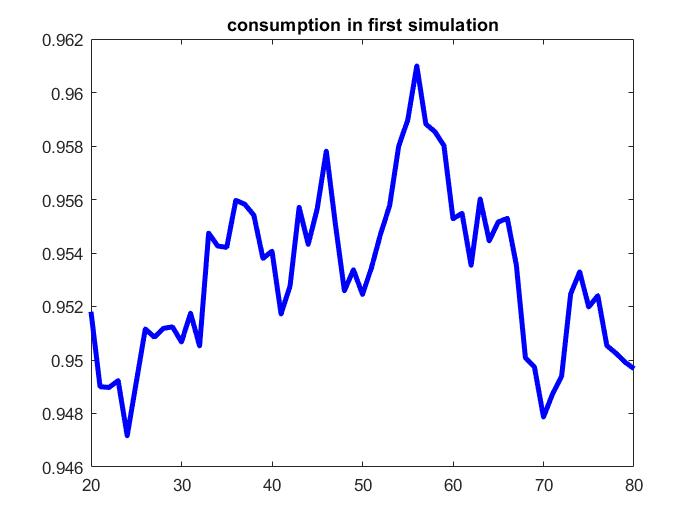
\includegraphics[width=\linewidth]{graphs/Q2/cons.jpg}
    %\caption{Coffee.}
  \end{subfigure}
  \begin{subfigure}[b]{0.32\linewidth}
      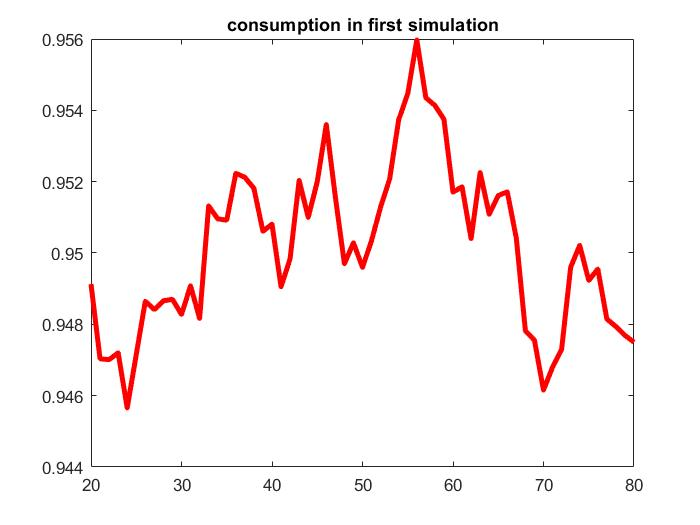
\includegraphics[width=\linewidth]{graphs/Q2/cons2.jpg}
      %\caption{More coffee.}
  \end{subfigure}
  \begin{subfigure}[b]{0.32\linewidth}
    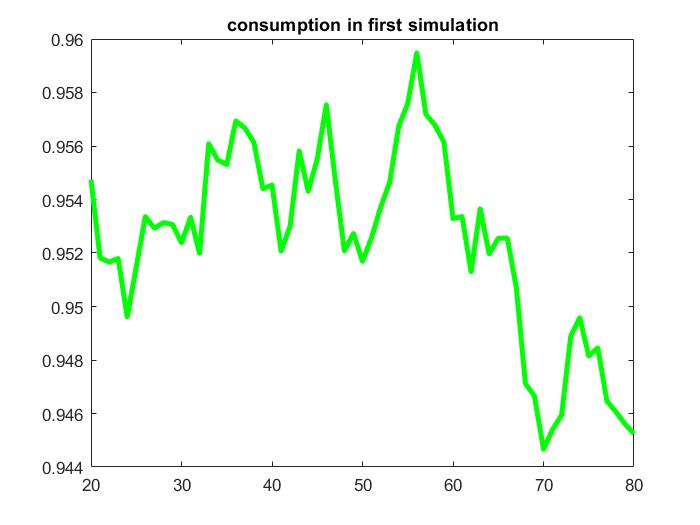
\includegraphics[width=\linewidth]{graphs/Q2/cons3.jpg}
      %\caption{More coffee.}
  \end{subfigure}
  \caption{Consumption in the first simulation}
    \label{fig:1}
\end{figure}

\begin{figure}[h!]
  \centering
  \begin{subfigure}[b]{0.32\linewidth}
    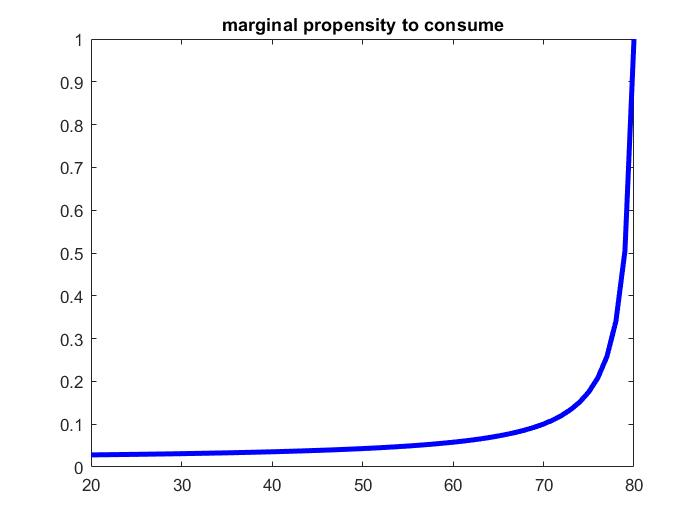
\includegraphics[width=\linewidth]{graphs/Q2/mpc.jpg}
    %\caption{Coffee.}
  \end{subfigure}
  \begin{subfigure}[b]{0.32\linewidth}
      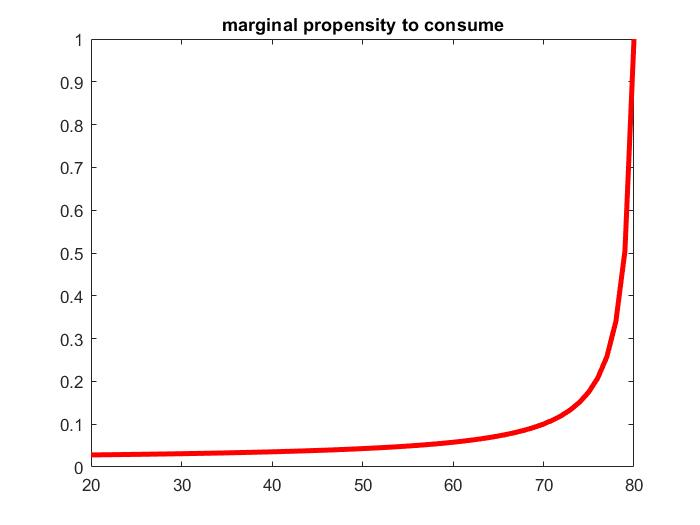
\includegraphics[width=\linewidth]{graphs/Q2/mpc2.jpg}
      %\caption{More coffee.}
  \end{subfigure}
  \begin{subfigure}[b]{0.32\linewidth}
    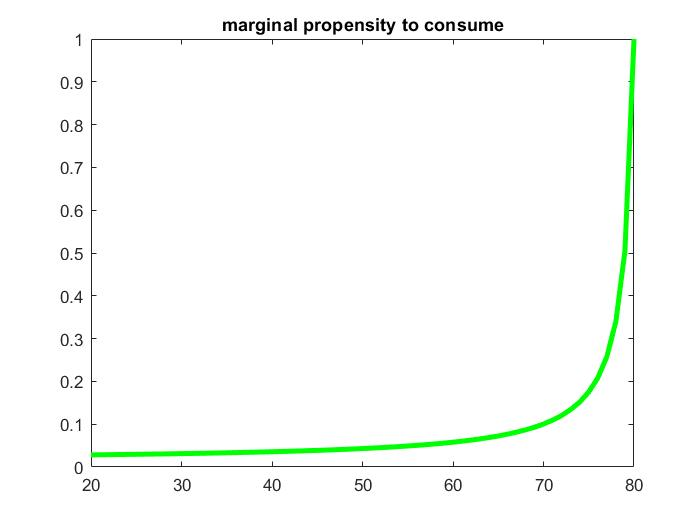
\includegraphics[width=\linewidth]{graphs/Q2/mpc3.jpg}
      %\caption{More coffee.}
  \end{subfigure}
  \caption{Marginal propensity of Consumption}
    \label{fig:2}
\end{figure}


\begin{figure}[h!]
  \centering
  \begin{subfigure}[b]{0.32\linewidth}
    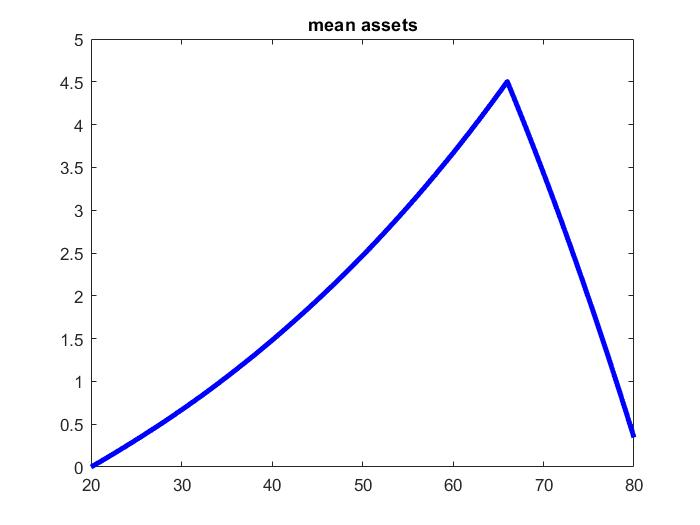
\includegraphics[width=\linewidth]{graphs/Q2/mean_asset.jpg}
    %\caption{Coffee.}
  \end{subfigure}
  \begin{subfigure}[b]{0.32\linewidth}
      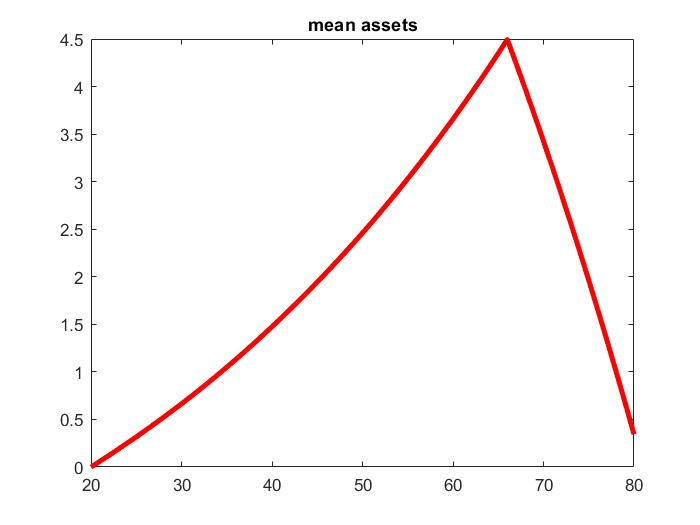
\includegraphics[width=\linewidth]{graphs/Q2/mean_asset2.jpg}
      %\caption{More coffee.}
  \end{subfigure}
  \begin{subfigure}[b]{0.32\linewidth}
    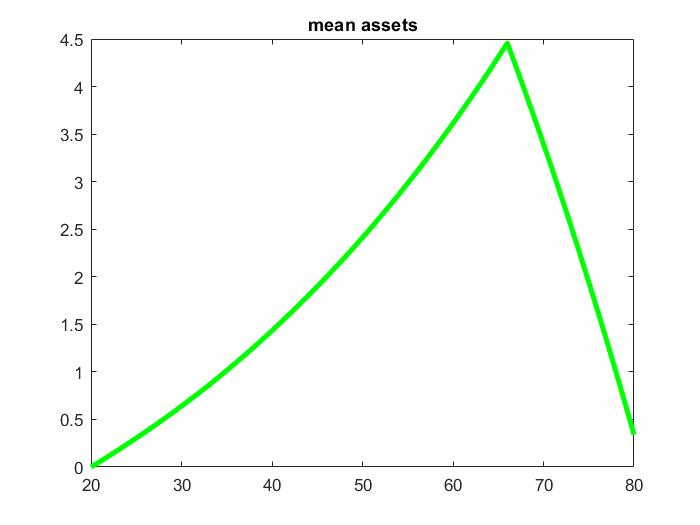
\includegraphics[width=\linewidth]{graphs/Q2/mean_asset3.jpg}
      %\caption{More coffee.}
  \end{subfigure}
  \caption{Mean assets holding}
    \label{fig:3}
\end{figure}

\begin{figure}[h!]
  \centering
  \begin{subfigure}[b]{0.32\linewidth}
    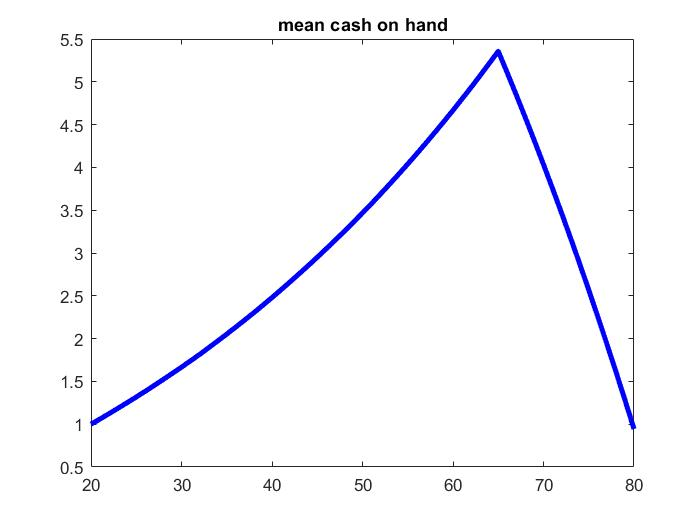
\includegraphics[width=\linewidth]{graphs/Q2/mean_x.jpg}
    %\caption{Coffee.}
  \end{subfigure}
  \begin{subfigure}[b]{0.32\linewidth}
      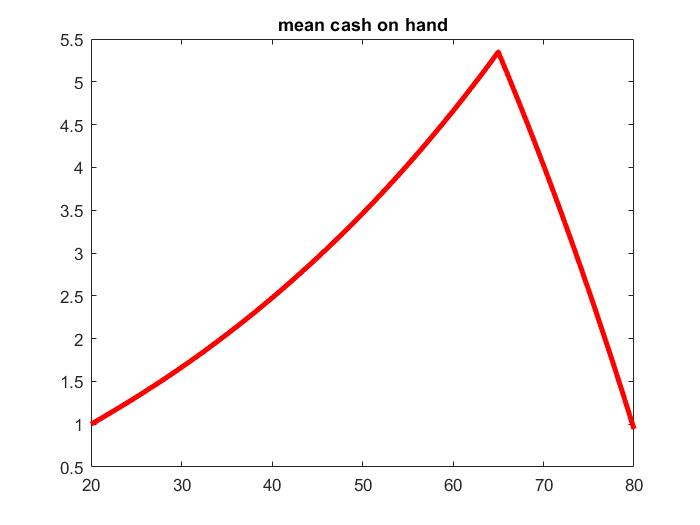
\includegraphics[width=\linewidth]{graphs/Q2/mean_x2.jpg}
      %\caption{More coffee.}
  \end{subfigure}
  \begin{subfigure}[b]{0.32\linewidth}
    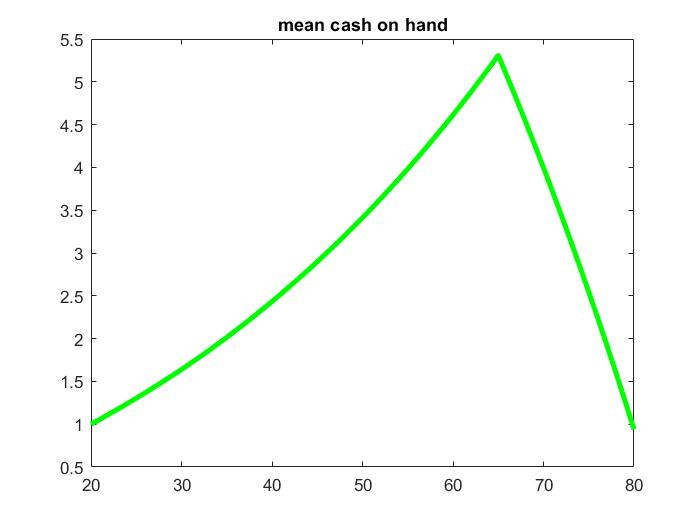
\includegraphics[width=\linewidth]{graphs/Q2/mean_x3.jpg}
      %\caption{More coffee.}
  \end{subfigure}
  \caption{Mean cash at hand}
    \label{fig:3}
\end{figure}

\begin{figure}[h!]
  \centering
  \begin{subfigure}[b]{0.32\linewidth}
    %\caption{Coffee.}
    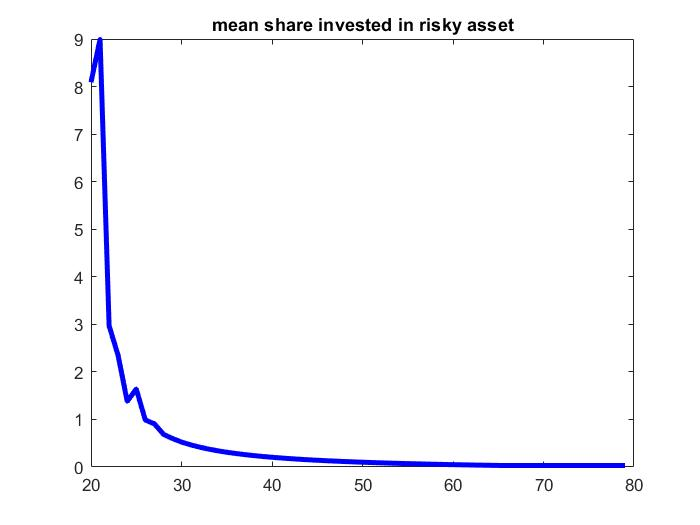
\includegraphics[width=\linewidth]{graphs/Q2/mean_share.jpg}
  \end{subfigure}
  \begin{subfigure}[b]{0.32\linewidth}
      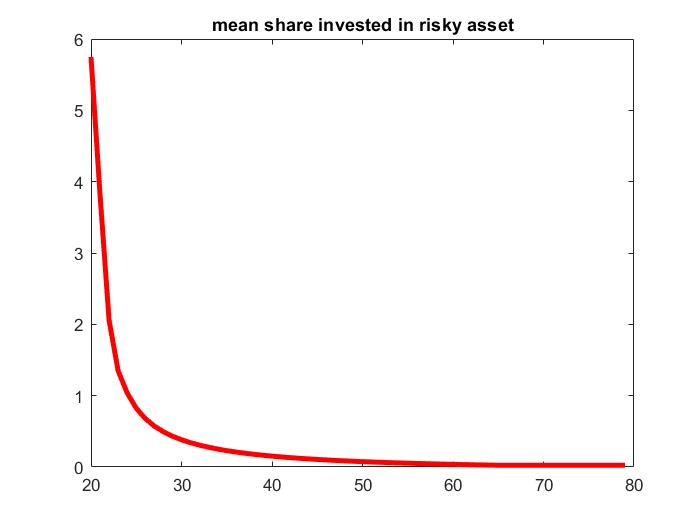
\includegraphics[width=\linewidth]{graphs/Q2/mean_share2.jpg}
      %\caption{More coffee.}
  \end{subfigure}
  \begin{subfigure}[b]{0.32\linewidth}
    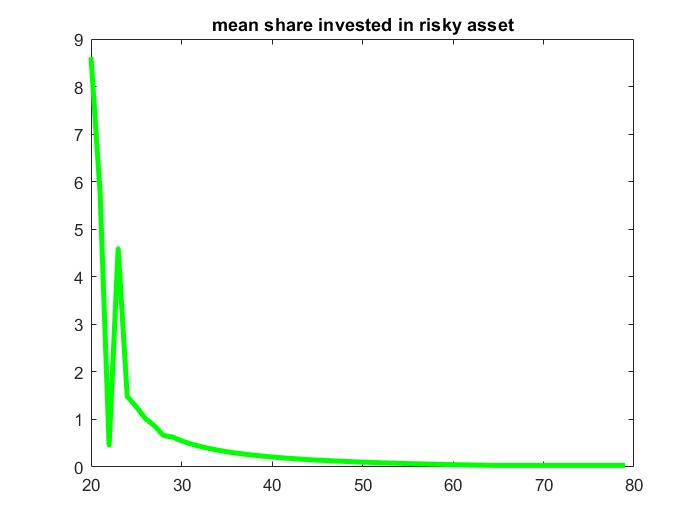
\includegraphics[width=\linewidth]{graphs/Q2/mean_share3.jpg}
      %\caption{More coffee.}
  \end{subfigure}
  \caption{Mean share of risky asset}
    \label{fig:4}
\end{figure}


\textbf{Q: What are the properties of consumption over the life-cycle and how do you interpret this path in light of the data features mentioned in the lecture?}

A: Agents accumulate assets (and cash-at-hand) before retiring and consume them fully before dying - note that in this context death is exogenous and non-stochastic. This implies that the marginal consumption of cash at hand increases over time. Consumption is highly volatile across the entire lifespan of the agent. It might be argued that consumption gets more volatile for older agents: young agents can dissave - knowing that, on expectation, they can save more later - and thus partially smooth consumption. On the other hand, older agents (that rely on a limited income and are dissaving their asset) cannot smooth consumption that easily.

\section*{Problem 1.3}

\textbf{Q: Relate the portfolio allocation for the case $\theta = 150$ and $\rho = 0.04$ to the "rule of thumb" advice of a fund manager who suggests to hold $\alpha_j = 1- \frac{j}{100}$ in stocks where $j$ is age.}

\begin{figure}[h!]
  \centering
  \begin{subfigure}[b]{0.49\linewidth}
    %\caption{Coffee.}
    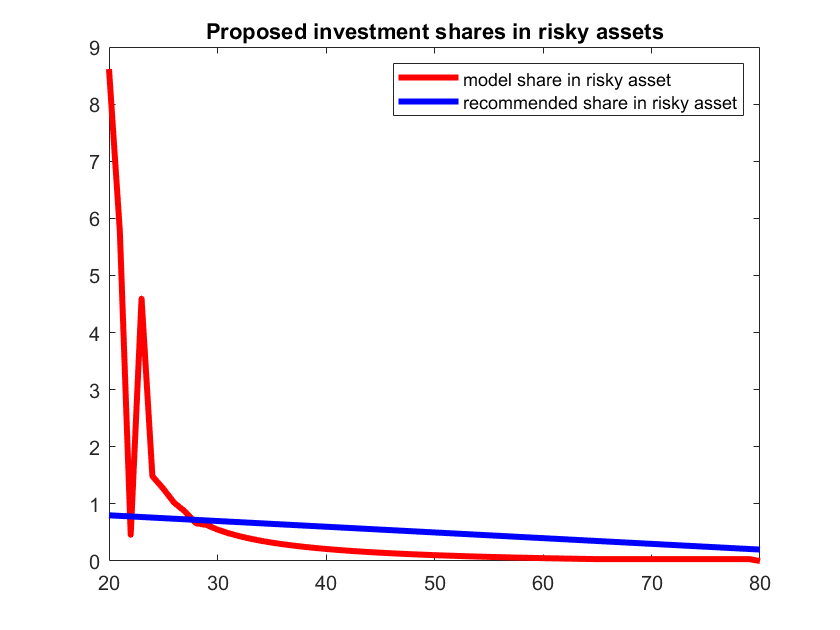
\includegraphics[width=\linewidth]{graphs/sharesriskyasset.png}
  \end{subfigure}
  \begin{subfigure}[b]{0.49\linewidth}
      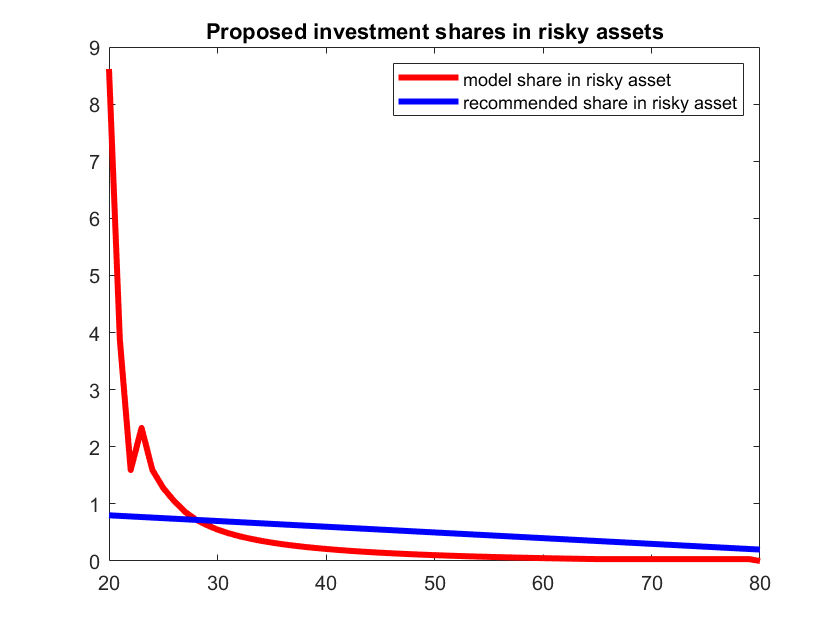
\includegraphics[width=\linewidth]{graphs/sharesriskyassetns100000.png}
      %\caption{More coffee.}
  \end{subfigure}
  \label{fig:5}
\end{figure}

Here $\rho$ is chosen to be rather large, leading to a lower $\beta$. This means, that people are more impatient and care relatively more about current consumption (or, expressed differently, care relatively less about future consumption).

Below, there is a graph comparing the recommended share in the risky asset to the estimated model prediction (obviously, this is based on our assumptions about how the returns/ incomes behave).

When we run the simulation \textbf{n = 100,000 times} the spike around age 23 becomes less negative\footnote{Note that the kink in some of the variables/ graphs above is because some very drastic shock realizations of the risky asset - it vanishes when we increase the number of simulations.}

This indicates, that the optimal shares predicted by the model will smooth out when n converges to infinity!

The proposed allocation is linear, which stands in contrast to the model findings. Also, according to the rule of thumb behavior, younger agents should invest in way less risky portfolios than they do in the model. On the other hand, old agents should invest in more risky assets than proposed by the model.

\section*{Problem 1.4}

a) The concept of inter-temporal substitution $\psi(c)=-\frac{\partial\frac{c2}{c1}}{\frac{c2}{c1}}\bigg(\frac{\partial\frac{1}{1+r}}{\frac{1}{1+r}}\bigg)^{-1}$, measures by how much percent the relative demand changes between periods as a reaction to a percentage change in prices. Since we have to solve an inter-temporal portfolio choice model, the setting is no longer static and becomes dynamic, the need to measure inter-temporal shifts and describes consumer's willingness to substitute consumption over time arises as not only risk aversion, but also inter-temporal substitution elasticity determine consumption decisions. With CRRA utility function, the two measures are just reciprocal of each other, $\theta=\frac{1}{\psi}$ and can therefore not be controlled separately. However, it is reasonable to choose a recursive utility function such as Epstein-Zin-Weil preferences as it helps us in overcoming this property by breaking the link between the parameters $\theta$ and $\psi$.    \\

b)

\textbf{Proof by backward induction}:

Investor's wealth evolves:
\begin{equation*}
    w_{t+1}=(w_t-c_t)R^{p}_{t+1}(\hat{\alpha_t})
\end{equation*}
Portfolio return is given by:
\begin{equation*}
  R^{p}_{t+1}(\hat{\alpha_t})=R^f+ \hat{\alpha_t}(R_{t+1}-R^f)
\end{equation*}
The optimization problem with Epstein-Zin-Weil utility function is given by:
\begin{equation*}
    U_t=\max\limits_{c_{t},\hat{\alpha}_{t},w_{t+1}}\bigg[ c_t^{1-\frac{1}{\psi}}+ \beta\bigg(\mathbb{E}_t\bigg[U^{1-\theta}_{t+1}\bigg]\bigg)^{\frac{1-\frac{1}{\psi}}{1-\theta}}\bigg]^{\frac{1}{1-\frac{1}{\psi}}}
\end{equation*}
Our guess is that the indirect utility function is given by $U_t=\gamma_t w_t$
, $\gamma_t$ captures dependence on time and state variables.
The indirect utility function is thus
\begin{equation*}
   U_t(w_t) = \bigg[ c_t^{1-\frac{1}{\psi}}+\beta\bigg(\mathbb{E}_t\bigg[\big(\gamma_{t+1}w_{t+1}\big)^{1-\theta}\bigg]\bigg)^\frac{1-\frac{1}{\psi}}{1-\theta}\bigg]^\frac{1}{1-\frac{1}{\psi}}\\
\end{equation*}
Using the resource constraint, we get:
\begin{align*}
     U_t(w_t)&=\bigg[ c_t^{1-\frac{1}{\psi}}+\beta\bigg(\mathbb{E}_t\bigg[\big(\gamma_{t+1}(w_t-c_t)R^{p}_{t+1}(\hat{\alpha}_t)\big)^{1-\theta}\bigg]\bigg)^\frac{1-\frac{1}{\psi}}{1-\theta}\bigg]^\frac{1}{1-\frac{1}{\psi}}\\
     &=\bigg[ c_t^{1-\frac{1}{\psi}}+\beta(w_t-c_t)^{1-\frac{1}{\psi}}\bigg(\mathbb{E}_t\bigg[\big(\gamma_{t+1}R^{p}_{t+1}(\hat{\alpha}_t)\big)^{1-\theta}\bigg]\bigg)^\frac{1-\frac{1}{\psi}}{1-\theta}\bigg]^\frac{1}{1-\frac{1}{\psi}}\\
     &=\bigg[ c_t^{1-\frac{1}{\psi}}+\beta(w_t-c_t)^{1-\frac{1}{\psi}}g\big(\gamma_{t+1}R^{p}_{t+1}(\hat{\alpha}_t)\big)^{1-\frac{1}{\psi}}\bigg]^\frac{1}{1-\frac{1}{\psi}}\\
     &=\bigg[ c_t^{1-\frac{1}{\psi}}+\beta(w_t-c_t)^{1-\frac{1}{\psi}}\Lambda_{t+1}\bigg]^\frac{1}{1-\frac{1}{\psi}}\\
\end{align*}

where g(.) is the certainty equivalent. From this we can rewrite the FOC for consumption as:
\begin{equation*}
    c_t^{-\frac{1}{\psi}}=\beta(w_t-c_t)^{-\frac{1}{\psi}}\Lambda_{t+1}
\end{equation*}
and thus:
\begin{equation*}
    c_t=(w_t-c_t)(\beta\Lambda_{t+1})^{-\psi}
\end{equation*}
and therefore:
\begin{equation*}
    c_t=m_t w_t
\end{equation*}
where:
\begin{equation*}
    m_t=\frac{1}{1+b_{t+1}},\hspace{2mm} \text{$for$} \hspace{2mm} b_{t+1}=(\beta\Lambda_{t+1})^\psi
\end{equation*}

Use this back in the objective to get:
\begin{align*}
     U_t(w_t) &= \bigg[ (m_tw_t)^{1-\frac{1}{\psi}}+\beta\bigg(\mathbb{E}_t\bigg[\big(\gamma_{t+1}(1-m_t)w_tR^{p}_{t+1}(\hat{\alpha}_t)\big)^{1-\theta}\bigg]\bigg)^\frac{1-\frac{1}{\psi}}{1-\theta}\bigg]^\frac{1}{1-\frac{1}{\psi}}\\
     &= \bigg[ (m_t)^{1-\frac{1}{\psi}}+\beta(1-m_t)^{1-\frac{1}{\psi}}\bigg(\mathbb{E}_t\bigg[\big(\gamma_{t+1}R^{p}_{t+1}(\hat{\alpha}_t)\big)^{1-\theta}\bigg]\bigg)^\frac{1-\frac{1}{\psi}}{1-\theta}\bigg]^\frac{1}{1-\frac{1}{\psi}}w_t\\
     &=\bigg[ (m_t)^{1-\frac{1}{\psi}}+\beta(1-m_t)^{1-\frac{1}{\psi}}\Lambda_{t+1}\bigg]^\frac{1}{1-\frac{1}{\psi}}w_t\\
     &=\bigg[ \bigg(\frac{1}{1+b_{t+1}}\bigg)^{1-\frac{1}{\psi}}+b_{t+1}^{\frac{1}{\psi}}\bigg(\frac{b_{t+1}}{1+b_{t+1}}\bigg)^{1-\frac{1}{\psi}}\bigg]^\frac{1}{1-\frac{1}{\psi}}w_t\\
     &=\bigg[ \bigg(\frac{1}{1+b_{t+1}}\bigg)^{1-\frac{1}{\psi}}+b_{t+1}\bigg(\frac{1}{1+b_{t+1}}\bigg)^{1-\frac{1}{\psi}}\bigg]^\frac{1}{1-\frac{1}{\psi}}w_t\\
     &=\bigg[ \bigg(\frac{1}{1+b_{t+1}}\bigg)^{1-\frac{1}{\psi}}(1+b_{t+1})\bigg]^\frac{1}{1-\frac{1}{\psi}}w_t\\
     &=\bigg(m_t^{-\frac{1}{\psi}}\bigg)^{\frac{1}{1-\frac{1}{\psi}}}w_t\\
     &= m_t^{-\frac{\frac{1}{\psi}}{1-\frac{1}{\psi}}}w_t.
\end{align*}
Hence the guess is verified, where $\gamma_t=m_t^{-\frac{\frac{1}{\psi}}{1-\frac{1}{\psi}}}$ and $m_t=\frac{c_t}{w_t}$

 Next, notice that:
\begin{equation*}
    g(\gamma_{t+1}R^{p}_{t+1}(\hat{\alpha}_t))=g(m_t^{-\frac{\frac{1}{\psi}}{1-\frac{1}{\psi}}}R^{p}_{t+1}(\hat{\alpha}_t))
\end{equation*}

which since $m_{t+1}=\frac{1}{1+b_{t+2}}$ we can rewrite by stochastic independence assumption as:
\begin{equation*}
     g\big((\gamma_{t+1}R^{p}_{t+1}(\hat{\alpha}_t))\big)=g(\gamma_{t+1})g\big(R^{p}_{t+1}(\hat{\alpha_t})\big)
\end{equation*}

Consequently, the FOC w.r.t $\hat{\alpha}_t$ by the chain rule of differentiation can be rewritten to the partial derivative

\begin{equation}\label{one}
    \pdv{\mathbb{E}\big[R_{t+1}^p(\hat{\alpha_t})^{1-\theta}\big]}{\hat{\alpha_t}}=0
\end{equation}

Let $\hat{\alpha_t}^{*}$ be the solution to equation \eqref{one}. In order to solve for  $\hat{\alpha_t}^{*}$, we use the approximation of $\mathbb{E}\big[R_{t+1}^p(\hat{\alpha_t})^{1-\theta}\big]$ given in  \textit{PFChoiceAPNotes}, which under log-normality of return can be approximated as:
\begin{equation*}
  \mathbb{E}\big[R_{t+1}^p(\hat{\alpha_t})^{1-\theta}\big] \approx  exp\bigg((1-\theta)\bigg(\mathbb{E}_t[ln(1+r^p_{t+1})]+(1-\theta)\frac{(\sigma_t^p)^2}{2}\bigg) \bigg)
\end{equation*}
Furthermore,
 $\mathbb{E}_t[ln(1+r^p_{t+1})]$ can be approximated as:
\begin{equation*}
    \mathbb{E}_t[ln(1+r^p_{t+1})]\approx \hat{\alpha_t}\mu_t +(1-\hat{\alpha_t})ln(1+r^f_{t+1})+\frac{1}{2}\hat{\alpha_t}(1-\hat{\alpha_t})\sigma_t^2.
\end{equation*}
Plugging this into the previous equation gives:
\begin{equation*}
 \mathbb{E}\big[R_{t+1}^p(\hat{\alpha_t})^{1-\theta}\big]\approx exp\bigg((1-\theta)\bigg(\hat{\alpha_t}\mu_t +(1-\hat{\alpha_t})ln(1+r^f_{t+1})+\frac{1}{2}\hat{\alpha_t}(1-\hat{\alpha_t})\sigma_t^2+(1-\theta)\frac{(\sigma_t^p)^2}{2}\bigg) \bigg)
\end{equation*}
where $\mu_t=\mathbb{E}_t[ln(1+r_{t+1})]$ is the conditional mean risky return. By this approximation, we can also approximate $(\sigma_t^p)^2$ as :
\begin{equation*}
    (\sigma_t^p)^2\approx\hat{\alpha}_t^2\sigma_t^2
\end{equation*}

Equation $\eqref{one}$ becomes:
\begin{equation*}
 \mu_t-ln(1+r^f_{t+1})+\frac{1}{2}(1-2\hat{\alpha}_t)\sigma^2+(1-\theta)\hat{\alpha}_t\sigma_t^2=0
\end{equation*}
Therefore, the approximation to household's investment decision, which is independent of time $t$, can be given as:
\begin{equation*}
    \hat{\alpha_t}^{*}=\frac{\mu_t-ln(1+r^f_{t+1})+\frac{1}{2}\sigma_t^2}{\theta\sigma_t^2}
\end{equation*}

Remember that:
\begin{equation*}
    b_{t+1}=(\beta\Lambda_{t+1})^\psi
\end{equation*}
For implementation on computer, $b_{t+1}$ can be rewritten as:
\begin{align*}
    b_{t+1} &= (\beta\Lambda_{t+1})^\psi\\
        &= \Bigg\{\beta \bigg(\mathbb{E}_t\bigg[\big(\gamma_{t+1}R^{p}_{t+1}(\hat{\alpha}_t^*)\big)^{1-\theta}\bigg]\bigg)^\frac{1-\frac{1}{\psi}}{1-\theta}\Bigg\}^\psi\\
        &= \bigg[\beta g(\gamma_{t+1})^{1-\frac{1}{\psi}}g(R_{t+1}^p(\hat{\alpha}_t^*))^{1-\frac{1}{\psi}}\bigg]^\psi
\end{align*}
where:
\begin{equation*}
  g(\gamma_{t+1})^{1-\frac{1}{\psi}}= \Bigg\{ \Bigg(\mathbb{E}_t\bigg[ \big(m_{t+1}^{-\frac{\frac{1}{\psi}}{1-\frac{1}{\psi}}}\big)^{1-\theta}\bigg]\Bigg)^{\frac{1}{1-\theta}}\Bigg\}^{1-\frac{1}{\psi}}=m_{t+1}^{-\frac{1}{\psi}}
\end{equation*}

\begin{align*}
  g(R_{t+1}^p(\hat{\alpha}_t^*))^{1-\frac{1}{\psi}}&= \Bigg\{ \Bigg(\mathbb{E}_t\bigg[ \big(  R_{t+1}^p(\hat{\alpha}_t^*)          \big)^{1-\theta}\bigg]\Bigg)^{\frac{1}{1-\theta}}\Bigg\}^{1-\frac{1}{\psi}}\\
  &= \Bigg\{ \Bigg(  exp\bigg((1-\theta)\bigg(\mathbb{E}_t[ln(1+r^p_{t+1})]+(1-\theta)\frac{(\sigma_t^p)^2}{2}\bigg)\bigg)      \Bigg)^{\frac{1}{1-\theta}}\Bigg\}^{1-\frac{1}{\psi}}\\
  &= exp\bigg(\bigg(1-\frac{1}{\psi}\bigg)\bigg(\mathbb{E}_t[ln(1+r^p_{t+1})]+(1-\theta)\frac{(\sigma_t^p)^2}{2}\bigg)\bigg)
\end{align*}

Putting all together yields:
\begin{equation*}
    b_{t+1}=m_{t+1}^{-1}\bigg[\beta  exp\bigg(\bigg(1-\textcolor{red}{\frac{1}{\psi}}\bigg)\bigg(\mathbb{E}_t[ln(1+r^p_{t+1})]+(1-\theta)\frac{(\sigma_t^p)^2}{2}\bigg)\bigg)\bigg]^{\textcolor{red}{\psi}}
\end{equation*}
The term colored in red is the difference from standard term when solving with CRRA utility.

At terminal date, we have:
\begin{align*}
    c_T&=w_T\\
    U_T&=c_T=w_T
\end{align*}
Given this, marginal propensity to consume at terminal date  \big($m_T=\frac{c_T}{w_T}$\big)  is 1. Having found optimal portfolio choice $ \hat{\alpha_t^*}$, we can simulate portfolio return for every period, and therefore can recursively solve for optimal $c_t$ and $w_t$ in every period $t$ using the expressions given previously:
\begin{align*}
    b_{t+1}&=m_{t+1}^{-1}\bigg[\beta  exp\bigg(\bigg(1-\frac{1}{\psi}\bigg)\bigg(\mathbb{E}_t[ln(1+r^p_{t+1})]+(1-\theta)\frac{(\sigma_t^p)^2}{2}\bigg)\bigg)\bigg]^{\psi}\\
    m_{t}&=\frac{1}{1+b_{t+1}}\\
    w_t^*&=\frac{w_{t+1}^*}{(1-m_t)R_{t+1}^p(\hat{\alpha}_t^*)}\\
    c_t^*&=m_tw_t^*\\
    \hat{\alpha_t}^{*}&=\frac{\mu_t-ln(1+r^f_{t+1})+\frac{1}{2}\sigma_t^2}{\theta\sigma_t^2}
\end{align*}
c) Results are given in matlab file.\\

d) when $\theta=\frac{1}{\psi}$, the red term in b) becomes the standard term when solving the model with CRRA utility function, therefore with the same terminal condition and other variables are the same, we get the same findings as yours.\\

e) when we set $\theta$ to the values from previous exercise for CRRA utility but let $\psi=0.5$, we can see that instead of $\psi=\frac{1}{\theta}=\frac{1}{150}$, which is very small in the case of CRRA preferences, now we have $\psi=0.5$ with EZW Preferences. When we look at the solution to the problem with CRRA and EZW preferences, we have that:
\begin{align*}
    b_{t+1}^{CRRA}&=m_{t+1}^{-1}\beta^{\frac{1}{\theta}}  exp\bigg(\bigg  (1-\theta\bigg)\frac{1}{\theta}\bigg(\mathbb{E}_t[ln(1+r^p_{t+1})]+(1-\theta)\frac{(\sigma_t^p)^2}{2}\bigg)\bigg)\\
     b_{t+1}^{EZW}&=m_{t+1}^{-1}\beta^\psi exp\bigg(\bigg(1-\frac{1}{\psi}\bigg)\psi\bigg(\mathbb{E}_t[ln(1+r^p_{t+1})]+(1-\theta)\frac{(\sigma_t^p)^2}{2}\bigg)\bigg)\\
\end{align*}
For $\psi>\frac{1}{\theta}$(which is the case), the exponential term of $b_{t+1}^{EZW}$ will be larger than that of $b_{t+1}^{CRRA}$; however, $\beta^\psi$ is smaller than $\beta^\frac{1}{\theta}$ as $0<\beta<1$. Suppose that the effect of the exponential term dominates that of $\beta$ such that for the same $m_T$ in the last day of agent's life, we expect $b_t^{EZW}>b_t^{CRRA}$, which means $m_t^{EZW}<m_t^{CRRA}$ for all $t$. Further more the gap between $m_t^{EZW}$ and $m_t^{CRRA}$ becomes even larger when we come to initial periods of agent's life as $m_t$ depends on $m_{t+1},...,m_T$. This means that with EZW preference, when the agent is so risk-averse that this even dominates the agent's preference for early consumption, he will consume less than in the case of CRRA preference in each period and shift his consumption towards later periods in his life.

Our simulation shows that, as expected, the agent behaviour does not change with CRRA or Epstein-Zin-Weil preferences such that $\psi=\frac{1}{\theta}$ (Figure \ref{fig:7} - \ref{fig:10}). Furthermore the simulation with $\psi = 0.5$ shows that agents consumption increases over time, reflecting the mechanism highlighted in the previous paragraph (Figure \ref{fig:7}). The agent reacts proportionally to the same interest rate shocks, albeit with a different intensity (Figure \ref{fig:8}) The increase in risk aversion affects also the amount of risky assets held by the agent (Figure \ref{fig:9}) and - therefore - returns, that are remarkably less volatile (Figure \ref{fig:10}).


\begin{figure}[h!]
  \centering
  \begin{subfigure}[b]{0.32\linewidth}
    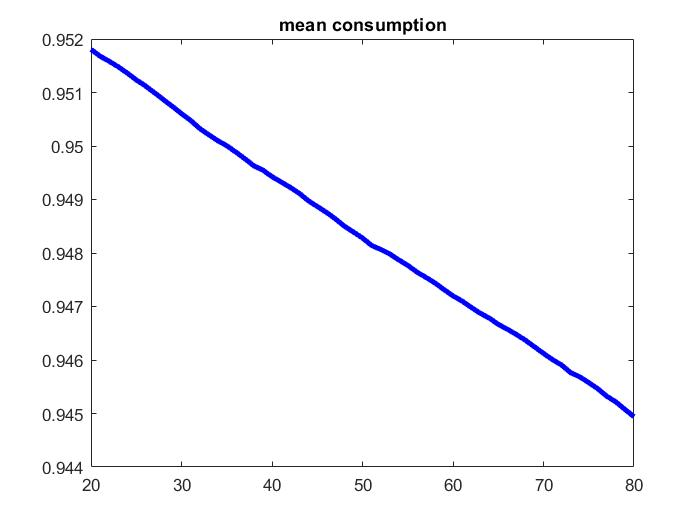
\includegraphics[width=\linewidth]{graphs/Q2/mean_cons.jpg}
    \caption{CRRA}
  \end{subfigure}
  \begin{subfigure}[b]{0.32\linewidth}
      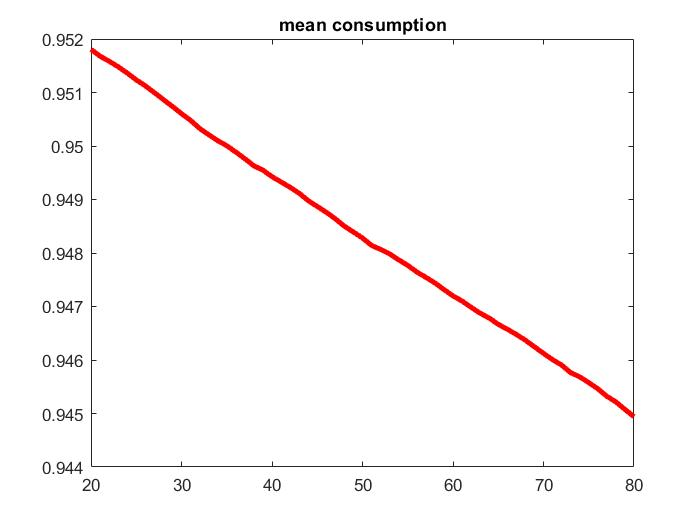
\includegraphics[width=\linewidth]{graphs/Q4/mean_cons_ezw--.jpg}
      \caption{EZW ($\psi = \frac{1}{\theta}$)}
  \end{subfigure}
  \begin{subfigure}[b]{0.32\linewidth}
    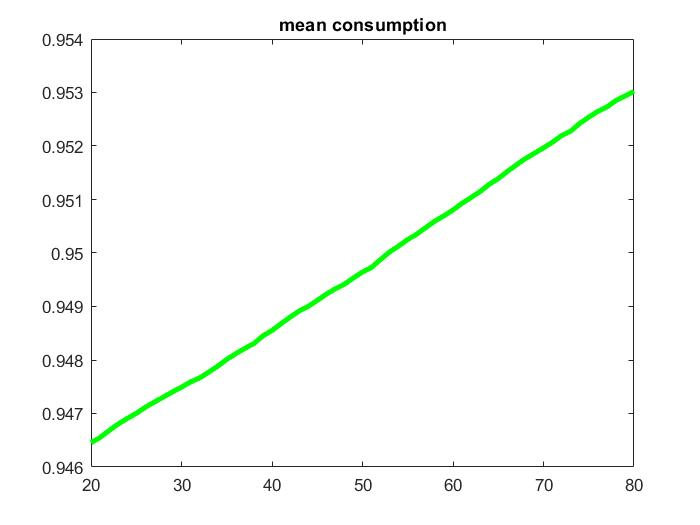
\includegraphics[width=\linewidth]{graphs/Q4/mean_cons_ezw.jpg}
      \caption{EZW ($\psi = 0.5$)}
  \end{subfigure}
  \caption{Mean consumption}
    \label{fig:7}
\end{figure}

\begin{figure}[h!]
  \centering
  \begin{subfigure}[b]{0.32\linewidth}
    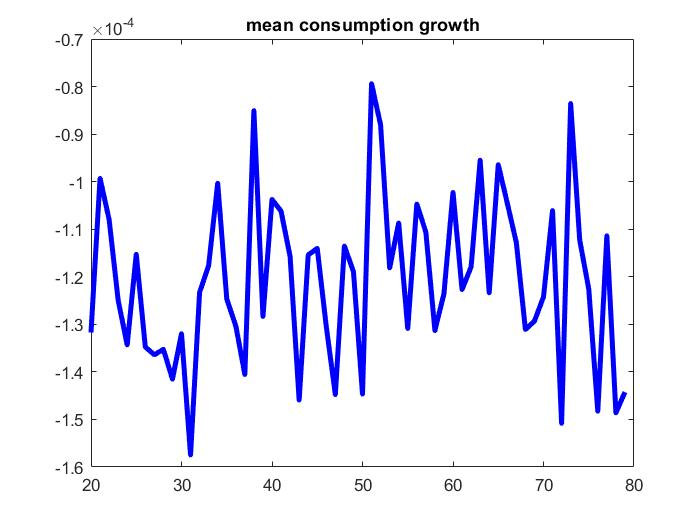
\includegraphics[width=\linewidth]{graphs/Q2/mean_cons_growth.jpg}
    \caption{CRRA}
  \end{subfigure}
  \begin{subfigure}[b]{0.32\linewidth}
      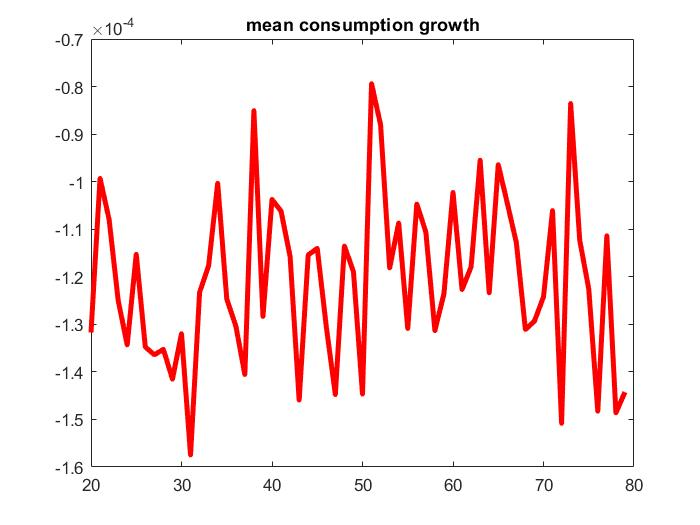
\includegraphics[width=\linewidth]{graphs/Q4/mean_cons_grow_ezw--.jpg}
      \caption{EZW ($\psi = \frac{1}{\theta}$)}
  \end{subfigure}
  \begin{subfigure}[b]{0.32\linewidth}
    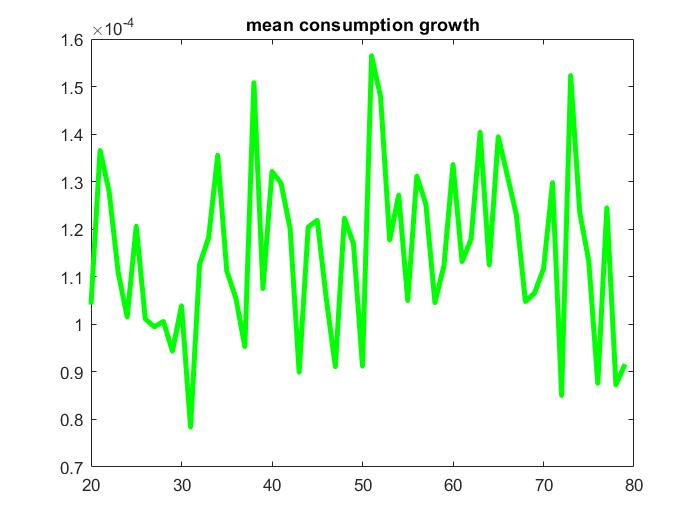
\includegraphics[width=\linewidth]{graphs/Q4/mean_cons_grow_ezw.jpg}
      \caption{EZW ($\psi = 0.5$)}
  \end{subfigure}
  \caption{Mean consumption growth}
    \label{fig:8}
\end{figure}

\begin{figure}[h!]
  \centering
  \begin{subfigure}[b]{0.32\linewidth}
    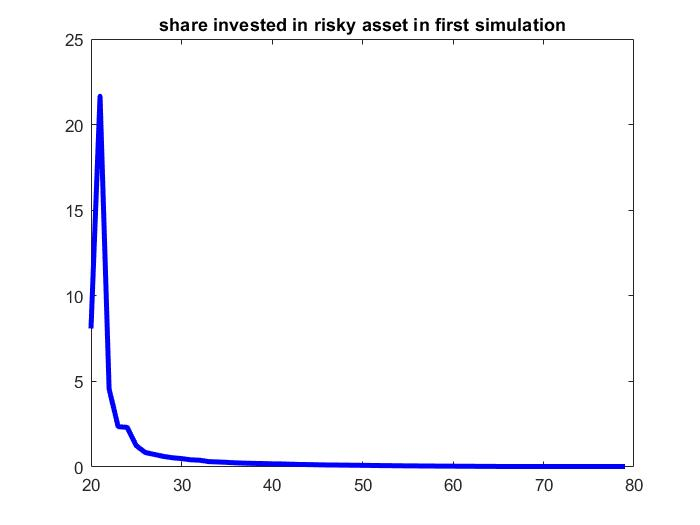
\includegraphics[width=\linewidth]{graphs/Q2/share.jpg}
    \caption{CRRA}
  \end{subfigure}
  \begin{subfigure}[b]{0.32\linewidth}
      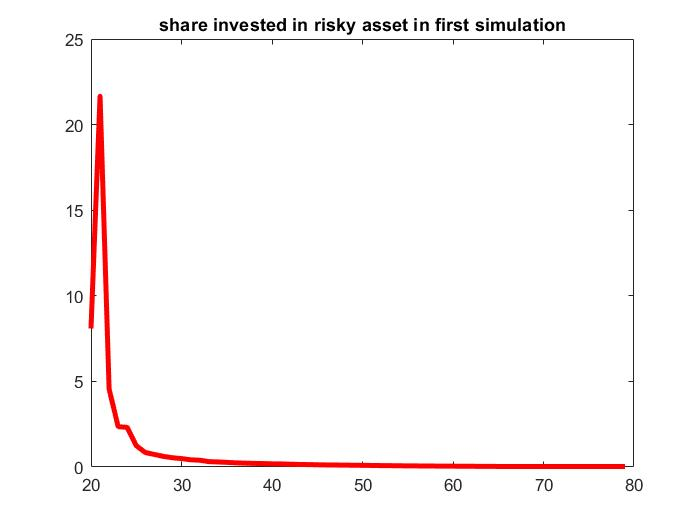
\includegraphics[width=\linewidth]{graphs/Q4/share_ezw--.jpg}
      \caption{EZW ($\psi = \frac{1}{\theta}$)}
  \end{subfigure}
  \begin{subfigure}[b]{0.32\linewidth}
    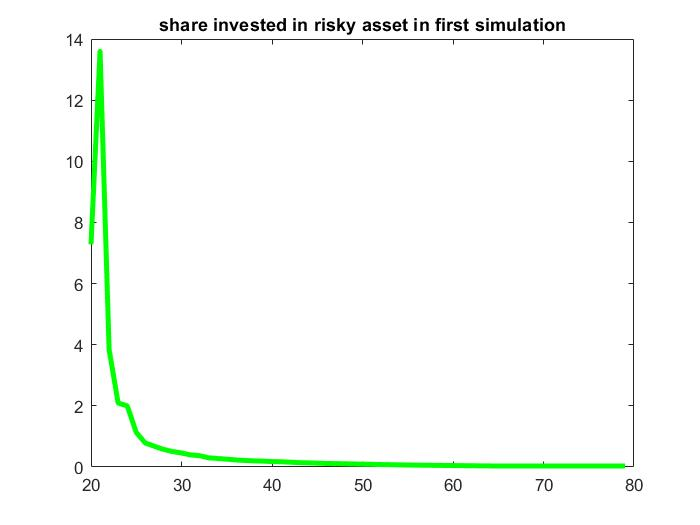
\includegraphics[width=\linewidth]{graphs/Q4/share_ezw.jpg}
      \caption{EZW ($\psi = 0.5$)}
  \end{subfigure}
  \caption{Share of risky assets}
    \label{fig:9}
\end{figure}

\begin{figure}[h!]
  \centering
  \begin{subfigure}[b]{0.32\linewidth}
    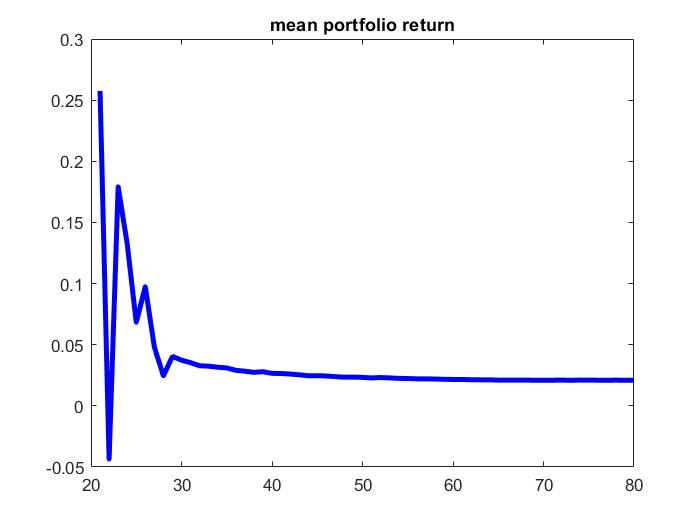
\includegraphics[width=\linewidth]{graphs/Q2/mean_ret.jpg}
    \caption{CRRA}
  \end{subfigure}
  \begin{subfigure}[b]{0.32\linewidth}
      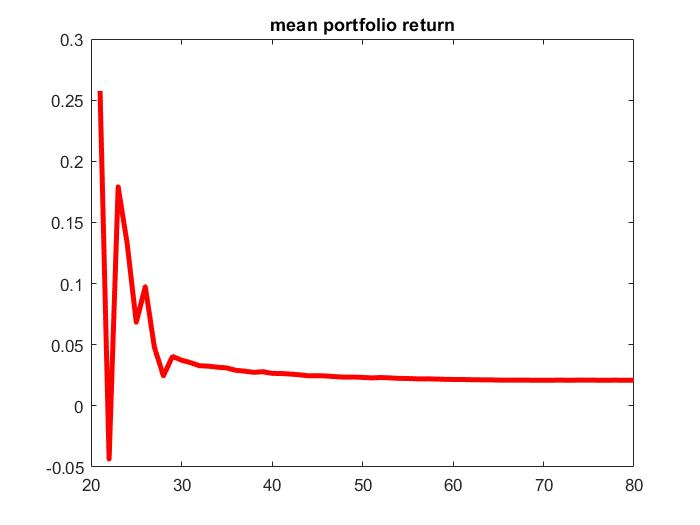
\includegraphics[width=\linewidth]{graphs/Q4/mean_ret_ezw--.jpg}
      \caption{EZW ($\psi = \frac{1}{\theta}$)}
  \end{subfigure}
  \begin{subfigure}[b]{0.32\linewidth}
    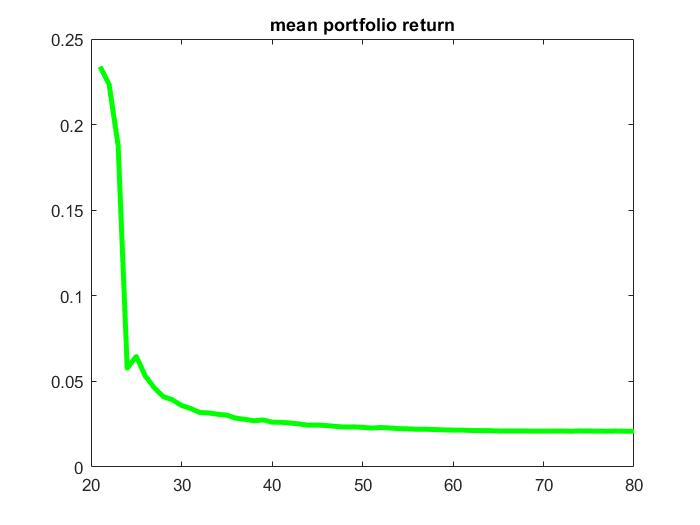
\includegraphics[width=\linewidth]{graphs/Q4/mean_ret_ezw.jpg}
      \caption{EZW ($\psi = 0.5$)}
  \end{subfigure}
  \caption{Mean portfolio return}
    \label{fig:10}
\end{figure}

\pagebreak

\section*{Problem 2}

Cocco et al (2005) investigate a finite horizon life cycle model of consumption and portfolio choice with non-tradable labour income which can be seen as a substitute for risk-free asset holdings and market incompleteness, in particular borrowing constraints, using realistic restrictions. Therefore, they estimate the labour income stream for different educational groups using the PSID, and find that its shape induces the agent to decrease his (proportional) asset holdings over time. Further, agents who face higher income risk hold smaller portfolio shares in equities such that income risk crowds out risk from holding assets. The crowding out effect becomes larger when the model allows for disastrous labour income draws. Additionally, the authors investigate the effect of endogenous borrowing constraints in their incomplete market setting. They find that the lower bound for the income distribution is key in determining borrowing capacity and portfolio allocation. Agents whose income process is bounded are faced with a positive endogenous borrowing constraint that induces the young to hold negative wealth and do not invest in equities. Lastly, the authors compute the utility cost associated with portfolio decisions that are not optimal and find that there is a substantial utility loss occurring from investing a constant share - which would be optimal under complete markets - and ignoring the labour income stream.


\end{document}
